\chapter{Einführung}

Die Komm.ONE entwickelte die letzten Jahre vor allem monolithische Anwendungen mit Java. Durch die Transformation zu einer moderneren Plattform die Containerisierung unterstützt bzw. darauf ausgelegt ist, sollen Anwendungen in einer Microservicearchitektur entwickelt werden. Als Pilotprojekt wird hierbei ein Modul der Anwendung WIBAS als Microservice implementiert und auf der neuen Plattform bereitgestellt.

Während die letzten Jahre die Anwendungen meist mithilfe von Java Webanwendungen (JSF/JSP) erstellt wurden, erhalten die modernisierten Anwendungen ein separates Frontend mithilfe eines JavaScript-Frameworks. Da viele Anwendungen neu geschrieben werden müssen, lohnt es sich Gedanken darüberzumachen wie die Frontend-Entwicklung nachhaltig und wiederverwendbar gestaltet werden kann.

In dieser Arbeit wird das Vorgehen und die Methodik beschrieben wie dies umgesetzt werden kann.

\chapter{Verwendete Technologien}

In der Neuentwicklung der Heimarbeit-Komponente wird im Frontend das Framework Angular (v14) verwendet. Angular ist ein komponentenbasiertes Frontend Typescript-Framework von Google, welches Open-Source entwickelt wird \cite{angular.17.01.2023}. Es wird sehr stark davon ausgegangen, dass in Zukunft vermehrt Angular eingesetzt wird. Die einzigen momentan verfügbaren Open-Source alternativen wäre React oder Vue.

In älteren Anwendungen die meist mithilfe von JSF (Jakarta Server Faces) geschrieben wurden, ist das CSS-Framework \textit{Prime} zum Einsatz gekommen (Primefaces). Dieses existiert für verschiedenste Technologien, unter anderem für Angular, React und Vue.

Prime soll auch für kommende Anwendungen weiterverwendet werden, es soll jedoch darauf geachtet werden, dass das Design einheitlich ist. Hierfür wurde vor dem Projektstart ein neuer Styleguide für die Komm.ONE entwickelt, der das Corporate Design beachtet und moderner wirkt.

Für die weitere Entwicklung kann davon ausgegangen werden, dass Prime weiterhin für ein Frontend-Framework eingesetzt wird und die Wiederverwendbarkeit soll auf der Ebene des CSS-Frameworks aufbauen. 

Ein wichtiges Tool hierfür ist das Themeing, welches Prime anbietet. Dabei ist die Grundstruktur und das Design des CSS-Frameworks voneinander getrennt und durch die Auswahl eines anderen Themes wird alles Grundlegende behalten, aber Abstände, Schriften und Farben werden angepasst. 

Ein einfacher Schritt der Wiederverwendbarkeit, wäre es ein eigenes Komm.ONE-Theme \textbf{einmal} zu schreiben und dies in neuen und ggf. auch alten Anwendungen einzubinden. Dabei ist das Endergebnis identisch, egal ob nun Angular, React, Vue oder JSF verwendet wird.

\chapter{Entwicklung eines Prime-Themes}

Ein Theme in Prime ist letztendlich eine große CSS-Datei mit Regeln für alle Komponenten. Ein neues Theme muss dabei nicht von $0$ geschrieben werden, sondern es kann ein schon vorhandenes Theme verwendet werden. Diese finden sich, wenn primeng installiert wurde, unter: \lstinline|node_modules/primeng/resources/themes/**/theme.css|. Dabei stehen 33 Themes kostenlos zur Verfügung \cite{Primeng.20.01.2023}. 

Um den Komm.ONE-Styleguide auf das Theme zu übertragen wurde zunächst im Projekt eine Demo-Seite erstellt. Auf dieser werden alle UI-Komponenten des Primeng-Frameworks gruppiert angezeigt. Um herauszufinden welche Styleklassen angepasst werden müssen, können mit den Entwicklertools im Browser die Abhängigkeiten nachgeschaut werden. Anschließend wurden die Klassen entsprechend der Stylevorgaben angepasst und im Ergebnis iterativ überprüft ob dieser mit den Vorgaben übereinstimmt und konsistent ist. 

Das am Ende vorliegende Theme kann nun in jeder Prime Anwendung verwendet werden um den Basis-Stil von Komm.ONE zu übernehmen. Dies funktioniert jedoch, nur wenn:
\begin{itemize}
    \setlength\itemsep{-1em}
    \item Das Prime-Framework richtig angewandt wird.
    \item Einzelne Komponenten nicht an anderer Stelle überschrieben werden
    \item Anwendungsspezifische Styles angepasst werden. 
\end{itemize}

Das Theme bietet nur einen stilistischen Rahmen, aber ein Grundlayout (Header, Sidebar, Footer, etc.) ist in Prime nicht vorgegeben und muss selbstständig aufgebaut werden. Da diese jedoch statisch sind, kann das Layout und der Style aus der Styleguide-Dokumentation (intern aufrufbar unter \href{https://confluence.komm-one.net/display/GWR/Styleguide+1.0.1-alpha}{Confluence}) entnommen werden.

\chapter{Komponentenbasierte Architektur}

In der GUI-Entwicklung wurde seit dessen Anfängen das MVC-Muster verwendet, mit dem Ziel die Daten einer Anwendung, deren Darstellung und die Nutzerinteraktionen die ausgeführt werden können abzugrenzen. Mit der Veröffentlichung von React.js, einer JavaScript-Bibliothek von Facebook, wurde die Frontend-Entwicklung stückweise neu definiert. 

React führte die \glqq Component Based Architecture\grqq{} (CBA) ein. Eine Methodik um individuelle Teilstücke einer Benutzeroberfläche in unabhängige Komponenten zu kapseln. 

Komponenten bauen auf dem Konzept von Ajax (Asynchronous JavaScript and XML) auf, bei dem Anfragen direkt von Client an den Server geschickt werden. Dadurch kann das DOM\footnote{Document Object Model; Das abstrake Model einer Webseite, das verwendet wird um diese zu rendern. JavaScript kann auf das DOM zugreifen und manipulieren um zur Laufzeit Änderungen vorzunehmen} dynamisch angepasst werden, ohne einen Reload der Seite hervorzurufen. In einer Komponente kann die Information welche Anfragen an den Server geschickt werden zusammen verkapselt werden. 

Der größte Vorteil von Komponenten ist die Wiederverwendbarkeit. Komponenten können einmal definiert werden und an mehreren Stellen mit anderen Metadaten verwendet werden. Da eine Grundregel der CBA die Unabhängigkeit der Komponenten ist. 

MVC teilt die Verantwortlichkeiten horizontal auf, CBA vertikal. Für MVC existieren Model, View und Controller und jede Funktionalität wird auf diese drei Verantwortlichkeiten aufgeteilt, während für CBA die Verantwortlichkeit auf Komponenten aufgeteilt wird. Design und Logik existieren alle auf demselben Level der Anwendung und Funktionalität erweitert sich mit der Implementierung neuer Komponenten \cite{dshaps.16.06.2016}.  

Durch React folgten viele neue CBA-Frameworks, unter anderem auch Angular. Angular hat den Vorteil, dass eine ganze Testumgebung mit installiert wird und auf Komponentenbasis Unit-Tests geschrieben werden können. Durch die grundlegende Unabhängigkeit zwischen Komponenten ist das Schreiben von Tests vereinfacht. 

\section{Entwicklung in der CBA (Angular)}

\subsection{Vorbereitung}
Zur Zeit der Entwicklung sollte die Datenstruktur (Klassendiagramme) stehen. Da Angular TypeScript verwendet, lohnt es sich TypeScript-Interfaces für eine konsistente und fehlerfreie Kommunikation mit dem Backend aufzubauen. Gleichzeitig müssen Services aufgebaut werden. Services bieten in Angular eine weitere Form der Abstraktion, wodurch Komponenten unabhängig voneinander werden. Sie \textit{bieten} eine Schnittstelle zum Backend an beliebig viele Komponenten an. Es lohnt sich die Schnittstellen des Backends - aufgeteilt in die Verantwortlichkeit der Datenobjekte - in Services zu übernehmen. 

\subsection{Test Driven Development}

Im Rahmen dieser Arbeit wurde das Test Driven Development (TDD) angewandt. Durch TDD werden zuerst Tests für die Anwendung geschrieben und danach die Implementierung. Dadurch passt sich die Implementierung der Tests (und damit meist den Use Cases) an und nicht umgekehrt.

\begin{figure}[H]
    \centering
    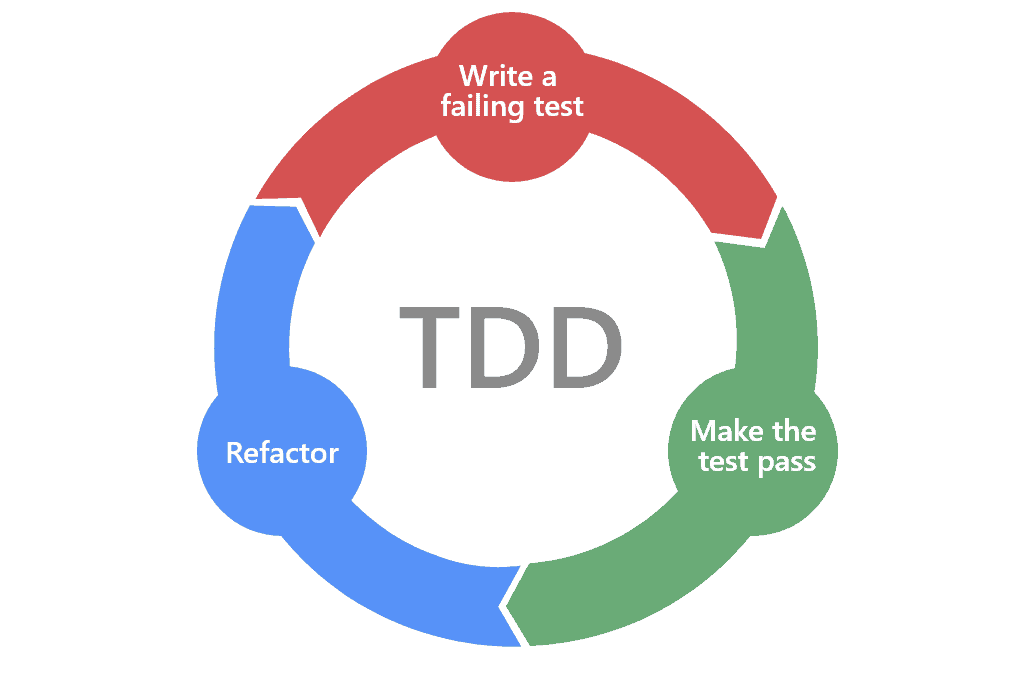
\includegraphics[width=0.8\textwidth]{images/test-driven-development-TDD.png}
    \caption{Test Driven Development}

\end{figure}    

Im Software-Engineering sollten alle Anforderungen einer Anwendung in Use Cases beschrieben sein. Meistens lässt sich jeder Use Case bzw. jede Gruppierung einer Verantwortlichkeit zu einer Komponente abkapseln. Dadurch können einzelne Use Cases für sich getestet werden und es kann sichergestellt werden, dass die Muss-Funktionalität umgesetzt wurde. Im Rahmen dieser Arbeit sollte sich dem Test Driven Development (TDD) bedient werden. Wenn das verwendete Test-Framework (im Normalfall bei Angular ist dies Jasmine) bekannt ist, ist dies auch sehr einfach möglich.

Ein minimales Setup (siehe Listing \ref{lst:testang}) besteht aus einer Testgruppe (describe) mit einer Setup-Funktion die vor jedem Unit-Test ausgeführt wird (beforeEach). Hier werden alle Mocks und Stubs vorbereitet, um diese vor jedem Test auf einen Ausgangspunkt zurückzusetzen. 

\begin{lstlisting}[language=JavaScript,caption={Minimaler Test einer Komponente},label=lst:testang]
describe('Testgroup', () => {
    let component: Component;
    let fixture: ComponentFixture<Component>;
    beforeEach(async () => {
    
      await TestBed.configureTestingModule({declarations: [Component]}).compileComponents();
        fixture = TestBed.createComponent(ResponsiblePersonComponent);
        component = fixture.componentInstance;
        fixture.detectChanges();
    });

    it('should create', ()=>{
        expect(component).not.toBeNull();
    })
});
\end{lstlisting}

Die einzelnen Unit-Tests folgen immer dem gleichen Schema, sofern diese keine anderen Abhängigkeiten besitzen:
\begin{enumerate}
    \item Komponente wird initialisiert (entweder durch das \lstinline|new| keyword, oder mithilfe eines TestBed)
    \item API der Komponente wird aufgerufen
    \item Erwartungen des öffentlichen Komponenten-States abfragen.
\end{enumerate}

Besitzt die Komponente jedoch einen Service als Abhängigkeit, ist es fast unumgänglich einen Mock oder Stub für diesen zu erstellen. Es sollte z. B. auch immer getestet werden, was passiert wenn die Backend-API einen Fehler zurückgibt und das muss im Frontend erzwungen werden. Genau für solche fälle unterstützt Angular die Dependency-Injection, in der Test-Vorbereitung kann nun ganz einfach ein Test-Service eingebunden werden, dieser sollte alle Funktionen unterstützen die in der tatsächlichen Umsetzung auch vorkommen. 

Wird z. B. auf die User-API zugegriffen, kann wie folgt (Listing \ref{lst:stubtest}) ein Service injected werden.

\begin{lstlisting}[language=JavaScript,caption={Injection eines Service-Stubs},label=lst:stubtest]
    const userStub = {
        getUser: ()=> return of({id:1,name:'name',...}),
        ...
    }
...
    await TestBed.configureTestingModule({
        declarations: [Component]
        providers: [{provide: UserService, useValue: userStub}]
        }).compileComponents();
...
    it('should load data correctly', ()=>{
        expect(component.user.name).toBe('name');
    })
\end{lstlisting}

Ein weiteres nützliches Tool ist das sogenannte \textit{Spying}. Manchmal können  die Abhängigkeiten ganz ohne Stubs genutzt werden, aber ein Service führt eine Aktion auf (z. B. das Loggen einer Nachricht). Die Funktionalität des Service muss beim Service getestet werden, nicht bei Komponenten die diesen aufrufen. Aber wenn sichergestellt werden soll, ob die Funktion überhaupt aufgerufen wurde, können Funktionen \textit{ausspioniert} werden.

\begin{lstlisting}[language=JavaScript,caption={Dependency Spying},label=lst:spytest]
...
    await TestBed.configureTestingModule({
        declarations: [Component]
        providers: [LogService]
        }).compileComponents();
    logService = TestBed.inject(LogService);
...
    it('should log something', ()=>{
        spyOn(logService, 'log');
        component.foo()
        expect(logService.log).toHaveBeenCalled();
    })
\end{lstlisting}

Als letzte wichtige Schnittstelle für Tests ist der Zugriff auf das DOM sehr wichtig. Im Allgemeinen sollte über e2e-Tests die wirkliche Nutzung abgedeckt werden, aber in Unit-Tests sollte überprüft werden, ob z. B. Tabellen-Zeilen erstellt werden mit den richtigen Daten, oder ob bei einer invaliden Eingabe eine Meldung angezeigt wird. Oder es können Knöpfe virtuell angeklickt werden um asynchrone Dialoge abzuschicken (meistens verwendet bei Bestätigungsdialogen).

\begin{lstlisting}[language=JavaScript,caption={Zugriff auf das DOM},label=lst:domtest]
    await TestBed.configureTestingModule({
        declarations: [Component]
        providers: [ConfirmationService]
        }).compileComponents();
...
    it('should do something', ()=>{
        component.foo(); // Oeffnet einen Bestaetigungsdialog
        const acceptBtn = fixture.debugElement.query(By.css('#accept-button'))
          .nativeElement as HTMLButtonElement;
        acceptBtn?.click();
        expect(...)...
    })
\end{lstlisting}

Mit diesem Stand können Tests aller Art geschrieben werden, um die Funktionalität einer Komponente sicherzustellen. Im Rahmen des Test Driven Development wurde dabei zunächst grundlegende Tests (Use Case Abdeckung \& Fehlerbehandlung) geschrieben und anschließend die Komponente implementiert mit dem Ziel, dass alle Tests erfolgreich durchlaufen \cite{Angular.02.02.2023}.

Am Ende wurde durch einen Code-Coverage Report analysiert welche Teile der Implementierung noch nicht getestet sind um ggf. nachzubessern. Das Ziel in diesem Projekt war es, eine Code-Coverage von 60 \% zu erreichen. Das heißt, 60 \% des Codes muss von einem oder mehreren Tests aufgerufen werden mit dem Ziel eine Behauptung in Verbindung mit diesem Aufruf zu testen.

\chapter{Fazit}

Die komponentenbasierte Entwicklung unterstützt die Wiederverwendbarkeit von Code. Technisch können einzelne implementierte Komponenten so wie sie sind, in andere Angular-Projekte kopiert werden. Es müssen nur die verwendeten Services im neuen Projekt angeboten werden. Die Möglichkeit der Wiederverwendung sagt jedoch nicht aus, dass der Code auch wiederverwendet wird, bzw. ob es Sinn ergibt diesen wiederzuverwenden.

Die Erstellung eines Prime-Theme z. B., oder eine Komponente, die eine Liste von Sachbearbeitern einer Fachanwendung auflistet, kann auch in weiteren Anwendung wiederverwendet werden. Es wird jedoch logischerweise immer Komponenten geben, die so spezifiziert auf die Anwendung sind, dass es keinen Wert hat eine Wiederverwendbarkeit anzustreben. Erst recht nicht, wenn die Rahmenbedingungen nicht geschaffen sind. 

Selbst wenn eine Komponente in einer anderen Anwendung innerhalb der Komm.ONE wiederverwendet werden könnte, ein anderes Entwicklerteam weiß wahrscheinlich nicht über bestehende Komponenten Bescheid und die Bemühungen nach eventuellen Bestandskomponenten zu forschen wäre es nicht wert. Es wäre also von Vorteil ein Rahmenwerk zu schaffen, um wiederverwendbare Komponenten auszutauschen, über einen Weg der über die Code-Repositorys hinaus geht und keine weiteren Sonderberechtigungen benötigt.